\pdfoutput=1 % ensure pdflatex (for arXiv)

\documentclass[11pt,a4paper]{article}
\usepackage[hyperref]{acl2020}
\usepackage{nert}
\usepackage{times}
\usepackage{latexsym}
\usepackage{dialogue}
\usepackage{graphicx}
\graphicspath{ {./images/} }
\usepackage{subfigure}
\usepackage{adjustbox}
%\renewcommand{\UrlFont}{\ttfamily\small}

% This is not strictly necessary, and may be commented out,
% but it will improve the layout of the manuscript,
% and will typically save some space.
\usepackage{microtype}

\aclfinalcopy % Uncomment this line for the final submission
%\def\aclpaperid{***} %  Enter the acl Paper ID here

%\setlength\titlebox{5cm}
% You can expand the titlebox if you need extra space
% to show all the authors. Please do not make the titlebox
% smaller than 5cm (the original size). 
% SOME CONFERENCES HAVE REJECTED SUBMISSIONS THAT VIOLATE THIS

\newcommand\BibTeX{B\textsc{ib}\TeX}

%\renewcommand{\nertcomment}[4]{\unskip}

\title{MakeCents: A Dialogue System for Coin Collectors}

\author{Ryan A. Mannion \\ Georgetown University \\ \eml{ram321@georgetown.edu}
}
\date{}

\begin{document}
\maketitle
\begin{abstract}
% Abstract: 5-6 sentences overviewing the project and contributions.
MakeCents is a chabot built with Rasa Open Source which is designed to be an easy-to-setup and easy-to-use interface that lets collectors interact with the PCGS online price guide. Additionally, this project releases tools for gathering coin data from PCGS's website. Following the principles of free and open-source software (FOSS), MakeCents and its counterpart, pcgs\_scraper, are well-documented with setup instructions, stable releases through GitHub, and issue tracking to help those in the future troubleshoot common issues. Participants in a brief survey reported that MakeCents often found what they were looking for, but that it could be hard to interpret for novice collectors.
\end{abstract}

\section{Introduction}
% Introduction: Describe the motivation behind the project and contributions.
Coin collecting is a fun and easy hobby, and can match the skill and resources of almost any collector. Beginners and long-time collectors alike often go "coin hunting," the process of looking for coins in common places like pocket change, the coin return tray of coin-counting machines, or basically anywhere else they can get their hands on coins for face value (i.e. the amount they are worth at a store). Knowing what can fetch more than its face value comes with time and experience, but even experienced coin collectors sometimes need to perform a sanity check to make sure the coin they are looking at is really worth something. 

MakeCents was built with coin hunters in mind: start up the chat dialogue with a few short keystrokes and MakeCents is ready to do all the heavy lifting; no more flipping through the pages of outdated coin price guides or having 10+ tabs open in the browser, MakeCents handles query requests and returns a price table for users to inspect so they can get back to looking at coins. 

MakeCents is built with \citeposs{bocklisch2017rasa} Rasa Open Source, allowing tech-savvy users to modify and update it with additional features in the future should they find something worth adding. This is a very likely scenario: much of the time building MakeCents was put into creating tools that are easy to use and which foster community participation, and as such the feature-set is currently limited to returning a picture of and prices for a single coin in table format. To that end, pcgs\_scraper -- the library responsible for getting the coin prices -- was developed in Python\footnote{Python Software Foundation. Python Language Reference, version 3.8. Available at \href{http://www.python.org}{http://www.python.org}} and released in a separate repository (more on this in \cref{sec:appr}).

% \section{Related Work}
% Related Work: What papers and projects in the community are similar to yours? Please cite them using ACL reference formatting. 

\begin{figure}[t!]
    \centering
    
\includegraphics[scale=0.3]{images/MakeCents_logo.png}
    \caption{MakeCents Logo}
    \label{fig:logo}
\end{figure}

\section{Approach}\label{sec:appr}
% Approach: What did you do and how did you do it?
The initial idea for MakeCents was to fetch coin prices with an API call, allowing for more time to develop other features like a way for collectors to interact with their own personal collections. Unfortunately, the only API for such a thing was deprecated in 2019. To solve this problem I decided to build my own library of tools to scrape prices from the website of a well-respected coin grading service, the Professional Coin Grading Service (PCGS)\footnote{\href{https://pcgs.com}{https://pcgs.com}}. PCGS certifies and grades coins on a scale from 1-70, enabling collectors to ensure the qulity of their coins and help fetch a higher price. PCGS also publishes a coin price guide based on PCGS-graded coins, which allows users to know approximately how much their coin could be worth. This guide was the perfect candidate for a price database for MakeCents. In order to allow others to have access to the same information, and to get updated information in the future, I packaged and released these tools under the name pcgs\_scraper.\footnote{The documented code is openly available at \href{https://github.com/ryanamannion/pcgs_scraper}{https://github.com/ryanamannion/pcgs\_scraper}}

pcgs\_scraper navigates PCGS's site tree and scrapes the information from thousands of coin listings, including mint year, where they were minted, denomination, designation, extra information (e.g. errors), links to images of that coin, and a narrative description of that coin's history. The resulting data structure from pcgs\_scraper is a free table, a list of dictionaries where each list item represents one coin, and each key:value pair is one of the above-mentioned features (e.g. year). The hope is that this data structure will allow others to easily incorporate data scraped from pcgs\_scraper into their projects. pcgs\_scraper also comes with its own query tool, and allows users to query the free table to find the coins they are looking for. Using pcgs\_scraper as the backend for MakeCents thus makes sense, as many of the basic features needed for the dialogue agent exist in some way in pcgs\_scraper. 

\begin{figure*}[t]
  \centering
  \subfigure{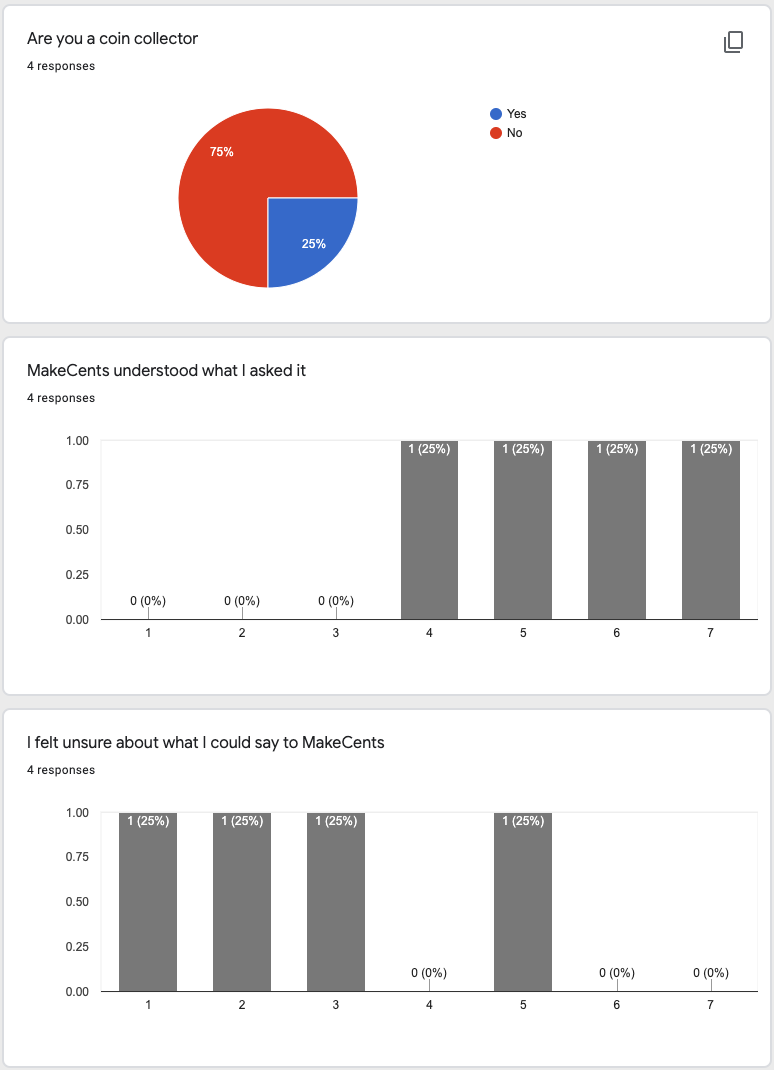
\includegraphics[scale=0.5]{images/results1.png}}\hfill
  \subfigure{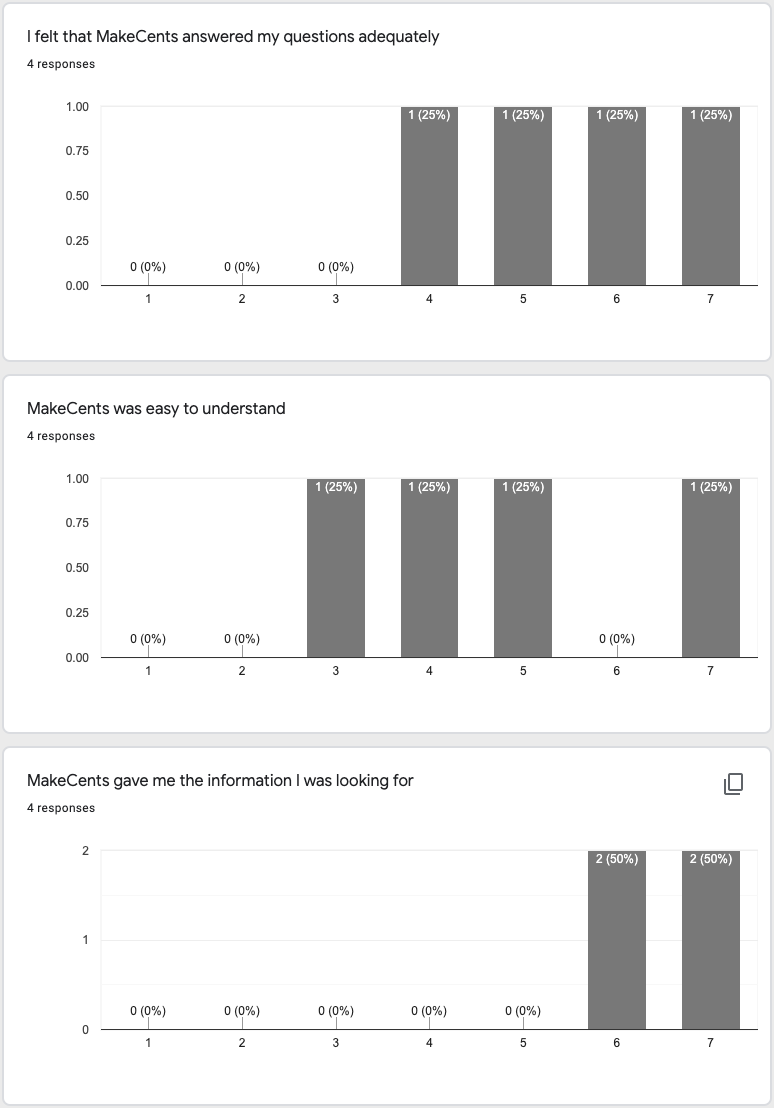
\includegraphics[scale=0.5]{images/results2.png}}
  \caption{Results from the MakeCents evaluation}
  \label{fig:results}
\end{figure*}

\subsection{Example Dialogue and Walkthrough}\label{subsec:ex}

Rasa offers two ways to test a bot which is still in development: running it in the shell, and running it in the closed-source Rasa X web interface. Below is an example conversation with MakeCents in its shell mode. For simplicity, the URLs for the coin image and the price table are rendered as images, but in the shell they would appear as hyperlinks.\footnote{Rasa X has issues with displaying local images, so the code submission for this paper has the table-as-png function turned off, see \href{https://github.com/ryanamannion/makecents/issues/1}{this GitHub issue}}

\begin{dialogue}
    \speak{User} Hello
    \speak{MakeCents} Hi! Welcome to MakeCents. I can help you quickly look for coin prices!
    \speak{MakeCents} You can get started by typing the name of any US coin! (e.g. 1909-S VDB Cent)
    \speak{MakeCents} TIP: Make sure to always include a year (YYYY) and a denomination (e.g. 1C, cent, penny, etc.). You can also specify the mint with a hyphen after the year (YYYY-M, e.g. 1909-S)
    \speak{User} What is the price of a 1997 penny?
    \speak{MakeCents} I found multiple results for your query.
    \speak{MakeCents} Please select the coin you would like to inspect:   (Use arrow keys) \\» 1: 1997 1C, RD \\\phantom{» }2: 1997-D 1C, RD
    \speak{User}1997 1C, RD
    \speak{MakeCents} \phantom{placeholder} \\ 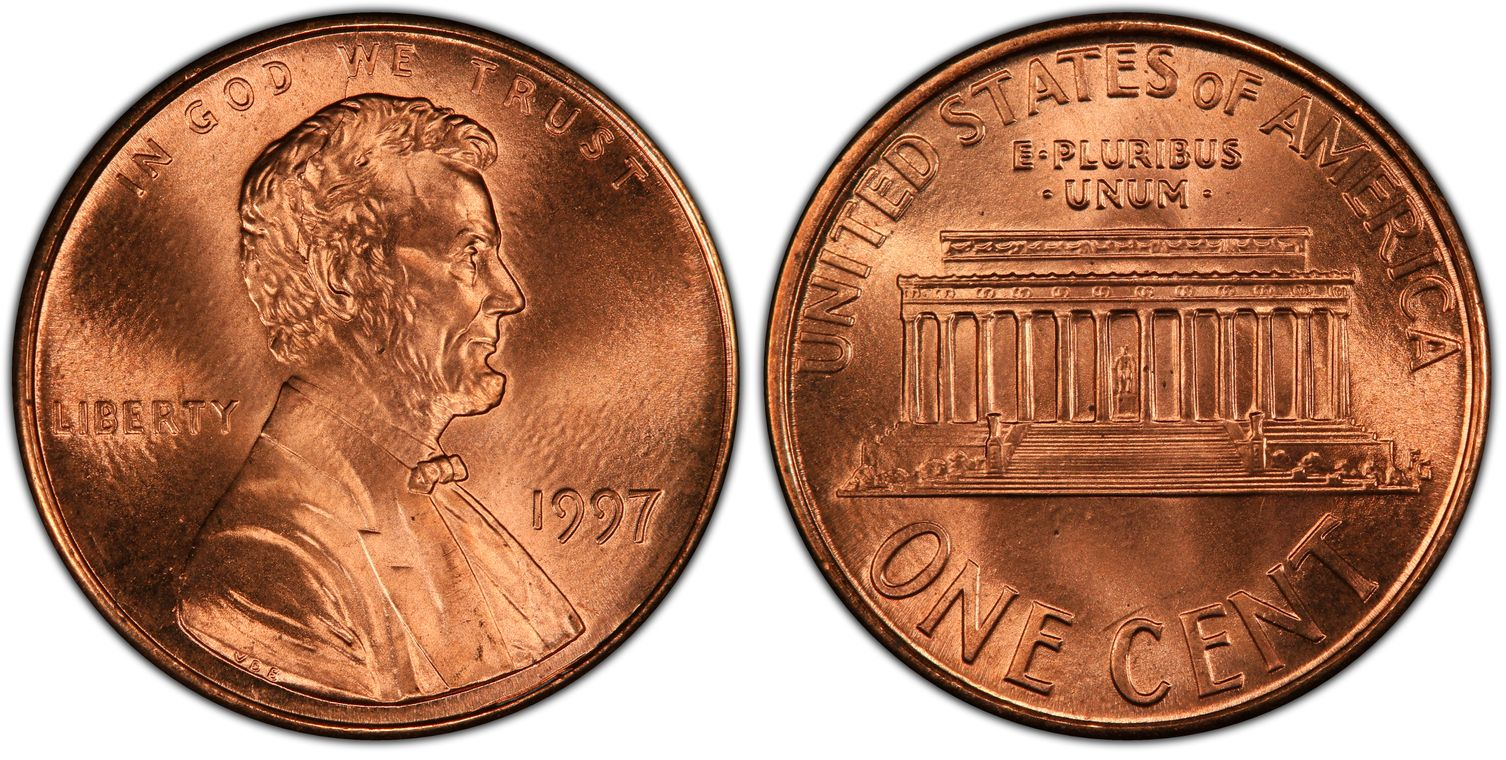
\includegraphics[scale=0.075]{images/19971c.jpg}\\ Here are the prices for 1997 1C, RD: \\
    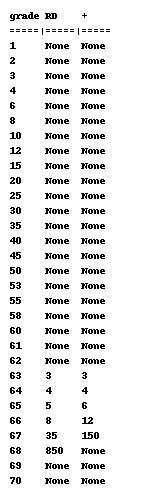
\includegraphics[scale=0.6]{images/price_table.png}
    \speak{User} Thank you!
    \speak{MakeCents} Of course!
    \speak{User} Bye
    \speak{MakeCents} Goodbye

\end{dialogue}

When Rasa classifies the user's intent as \verb|coin_query|, a custom action that runs pcgs\_scraper is launched. \verb|action_return_price| takes the user's input and validates it as having the two most crucial aspects of a coin query: a year and a denomination. This is usually able to limit the user's choices to around 2-5 options, depending on the year and number of variations for that denomination. If pcgs\_query returns more than one coin for a user's query, \verb|action_return_price| displays buttons which are ordered based on Levenshtein edit distance from the query, prompting the user to select a coin. The payload of the button is the exact description of the coin, which is in turn classified as a \verb|coin_query| intent again. This simplifies the Rasa custom action code, and allows pcgs\_query -- which already has functions for querying -- to do the heavy lifting in the back-end.

\section{Experiment}

Four participants took part in a short demo with MakeCents before responding to a questionnaire of eight questions designed to gauge user comfort and MakeCents' performance. The questions and their response types are listed in \Cref{tab:questions}.

Users' messages were relayed to MakeCents through video conferencing faithfully, and no direction was given to users other than what they might read in the README. Non-coin-collectors who asked about what coins they could query were instructed to find some change lying around and to query those coins, as that is part of the intended use case for the system.

\begin{table}[ht]
    \centering
    \small
    \begin{tabular}{p{0.75\linewidth} p{0.25\linewidth}}
        \toprule
        \textbf{Question} & \textbf{Response Type} \\
        \midrule
        I am a coin collector & Yes/No \\
        \midrule
        MakeCents understood what I asked it & Likert 1-7 \\
        \midrule
        I felt unsure about what I could say to MakeCents & Likert 1-7 \\
        \midrule
        I felt that MakeCents answered my questions adequately & Likert 1-7 \\
        \midrule
        MakeCents was easy to understand & Likert 1-7 \\
        \midrule
        MakeCents gave me the information I was looking for. & Likert 1-7 \\
        \midrule
        I would use MakeCents again in the future & Likert 1-7 \\
        \midrule
        If you have any other feedback, you can enter it here & Free \linebreak response \\
        \bottomrule
    \end{tabular}
    \caption{Questions from MakeCents evaluation Questionnaire}
    \label{tab:questions}
\end{table}


\section{Results}\label{sec:results}
% Results: What results did you find?
The results in \cref{fig:results} are sparse, given that only four participants were able to participate and respond to the form following a demo. One participant indicated that they were a coin collector.\footnote{I made posts to coin collecting forums like Reddit, but unfortunately did not receive any volunteers to test MakeCents}

Overall, the results show that MakeCents tended to understand and give the users what they asked for, with the responses to those questions all being 4 or above. Users also indicated that MakeCents tended to adequately answer their questions.

Some users indicated feeling unsure about what to ask MakeCents, and that MakeCents was not easy to understand at times. In response to the question asking if they would use MakeCents again, two users responded with a 6 and two with a 7. 

In the free-response section, one user wished that MakeCents did a better job at telling them what they could do, and suggested MakeCents say something before the user begins with "Hello." The user who indicated being a coin collector said that the pictures were a nice touch, but that the price table may be a bit hard to understand for beginner collectors. One final user indicated they wished they knew more about coins.

\section{Discussion}
% Discussion: What are the impacts of your results?
The results show that MakeCents still has a long way to go before a novice user can log in and begin evaluating coin prices. The hiccups users faced in their demos were mostly related to the way MakeCents communicated to them: the non-coin collectors all needed instruction on what coins they could query. These users were eventually instructed to find some change lying around and to look them up, but before that users asked questions like: \textit{What is the most expensive half dollar?} and \textit{What years were Sacagawea dollars minted?} These sorts of queries were out of scope for MakeCents in its current form, but led to the conclusion that a system for coin collectors and a system of lay people and beginners may look very different, and incorporating aspects of both into one system would make for a much more robust and usable dialogue agent.

Another anecdote from demonstrations was that users who were not coin collectors had a hard time interpreting the resulting price table. While it might be nice for advanced users to see that a lower-grade coin of a certain type is not worth keeping, users expressed being confused at why the price table was full of None values. A solution to this may be to incorporate a natural language generation component which synthesizes the results table into a sentence or two, and users can opt-in to seeing the entire table.

The results showed that user feedback is an invaluable step to developing a dialogue system, as you never know what users will say until you give them the opportunity (even though you THINK you might know). 

\section{Conclusion}
% Conclusion: Conclude the report with final thoughts and avenues for future work
The primary goal of this project -- to create a dialogue system to quickly access coin prices which is easy to setup and use -- was achieved, albeit with major revisions that need addressing before Makecents could be adopted by novice or non-technically savvy users. 

This project relied heavily on forum posts and documentation to get it to where it is, and it was important to me to contribute to the FOSS community as well. MakeCents and pcgs\_scraper are documented heavily, and all issues are tracked with cross-references to forum posts and commit hashes so other developers can benefit from my hard work as much as I benefitted from others.

This project was a learning experience for me, and I am grateful for the fun I had putting it together. Some things I learned included image manipulation with Python, bash scripting, a deeper understanding of Rasa and web scraping, issue tracking, making a repository look professional, and much more. 

\subsection{Future Work}
It is clear from the demonstration in \cref{subsec:ex} and the results in \cref{sec:results} that MakeCents is more suited -- at this stage at least -- for users who have at least a minimal understanding of coin collecting practices. For example, users are expected to understand the difference between a 1997 1C and a 1997-D 1C, the difference being that the latter was minted in Denver. MakeCents does have a response where it tells the user to consult the PCGS grading standards\footnote{available at \href{https://www.pcgs.com/grades}{https://www.pcgs.com/grades}}, but I would like to bake a bit more information into the system. PCGS does have a glossary of terms, which could be scraped and implemented.

I would also like to incorporate intents and responses that have to do with the scraped narratives from PCGS's CoinFacts pages. Users could ask for a history of the coin they query and MakeCents could pull information from there. 

There are many ways to go with this project from here, and I am excited to keep working on it


\bibliography{mypaper}
\bibliographystyle{acl_natbib}

% \appendix

\end{document}
